%% 10 - IMPORTS

\documentclass{scrartcl}
\usepackage{graphicx} % Required for inserting images

\usepackage[ngerman]{babel}
\usepackage[T1]{fontenc}        
\usepackage{amsmath}            
\usepackage{amsfonts}           
\usepackage{relsize}            %makes changing size in text possible
\usepackage[per-mode=symbol]{siunitx}


\graphicspath{ {./img/} }       %sets graphicspath to img folder

%% 20 - HEADER

\title{Projektvorstellung \\[0.2em]\smaller{} Simulation eines Airsoft Projektils}

\subtitle{A6P - Modellbildung und Simulation 2 \\ SoSe 2023}

\author{Philipp Kruppe, Maximilian Goldschmidt, Maximilian Reichhoff}

\date{\today}

\begin{document}

\maketitle

\vspace{20mm}

%% 30 - TABLE OF CONTENTS

\tableofcontents

\newpage

%% 40 - TEXT BODY

\section{Einleitung}

In der Ausarbeitung soll die Flugbahn eines Airsoft Projektils simuliert werden. 
Orientiert wird sich dabei an den technischen Daten einer Action Army AAP-01 Assassin Airsoft Pistole. \\
Die Simulation soll mehrstufig aufgebaut werden und soll die Eingabe von Parametern anderen Softairwaffen zulassen. 
Ebenfalls sollen die Parameter wie Wind, Starthöhe und -winkel geändert werden können.

\section{Ansatz für Modellbildung}

Zuerst wird ein Grundgerüst für Eingabe und Ausgabe von Werten und Ergebnissen im Matlab App Editor angelegt.
Die darauffolgende Modellbildung wird nach Fertigstellung des Grundgerüsts schrittweise hinzugefügt.
Zunächst im zweidimensionalen Raum und final in einem dreidimensionalen Modell.
Das Grundgerüst wird von Anfang für drei Dimensionen ausgelegt werden.\\
So kann auch der Einfluss der einzelnen Faktoren auf das vorherige Modell sichtbar gemacht werden.
Würde man alle Einflussgrößen auf die BB-Kugel vernachlässigen, würde es sich hierbei um einen schrägen Wurf handeln. \\
Da allerdings der Magnuseffekt und andere Effekte, die aus der Interaktion mit der Umgebungsluft auftreten und simuliert werden, ist ein schräger Wurf eine zu starke Vereinfachung. \\
Die Haupteinflussgröße für die Berechnung ist der Magnuseffekt der das Projektil so stark beeinflusst, dass die Flugbahn nicht mehr einem traditionellen schrägen Wurf ähnelt.
Mit einem einstellbarem Rad in der Pistole kann der Lauf stellenweise einseitig verengt werden. 
Dadurch erfährt die Kugel eine rückwärtsgerichtete Rotation um ihre Querachse. 
Diese Drehung kombiniert mit einem eintretendem Luftstrom resultiert in eine rechtwinklig auf dem Geschwindigkeitsvektor liegende Kraft.

\subsection{Einflussfaktoren}

Einflussfaktoren sind: 
\begin{itemize}
  \item Gravitation
  \item Energie der die Kugel am Startzeitpunkt
  \item Rotationsgeschwindigkeit der Kugel
  \item Größe und Masse der Kugel
  \item Luftwiderstand und der Abschusswinkel
  \item Windgeschwindigkeit und Richtung
\end{itemize}

\subsubsection{Physikalische Größen}

Die Gravitation als physikalische Größe ist fest vorgegeben und wird mit \SI{9.81}{\metre\per\square\second} veranschlagt. 
Die Kraft, mit der die Kugel abgeschossen wird, berechnet sich aus der Energie, die über den Druck der Pistole sowie das zugehörige Volumen des Zylinders vorgegeben ist. 
Die Standardgröße einer BB-Kugel beläuft sich auf sechs Millimeter. 
Das Gewicht der im Handel erhältlichen Kugeln variiert zwischen \num{0.20} bis \num{0.49} Gramm. \\
Die Kraft des Luftwiderstandes wird mit der Formel (5) berechnet. Für die benötigten Werte soll sich an Vorgaben der Umgebung orientiert werden. ($c_{w}$ einer Kugel = 0.45, Umgebungsdruck $\rho_{Luft} = 1.01325 hPa$)

\begin{figure}
    \centering % Zentrieren
    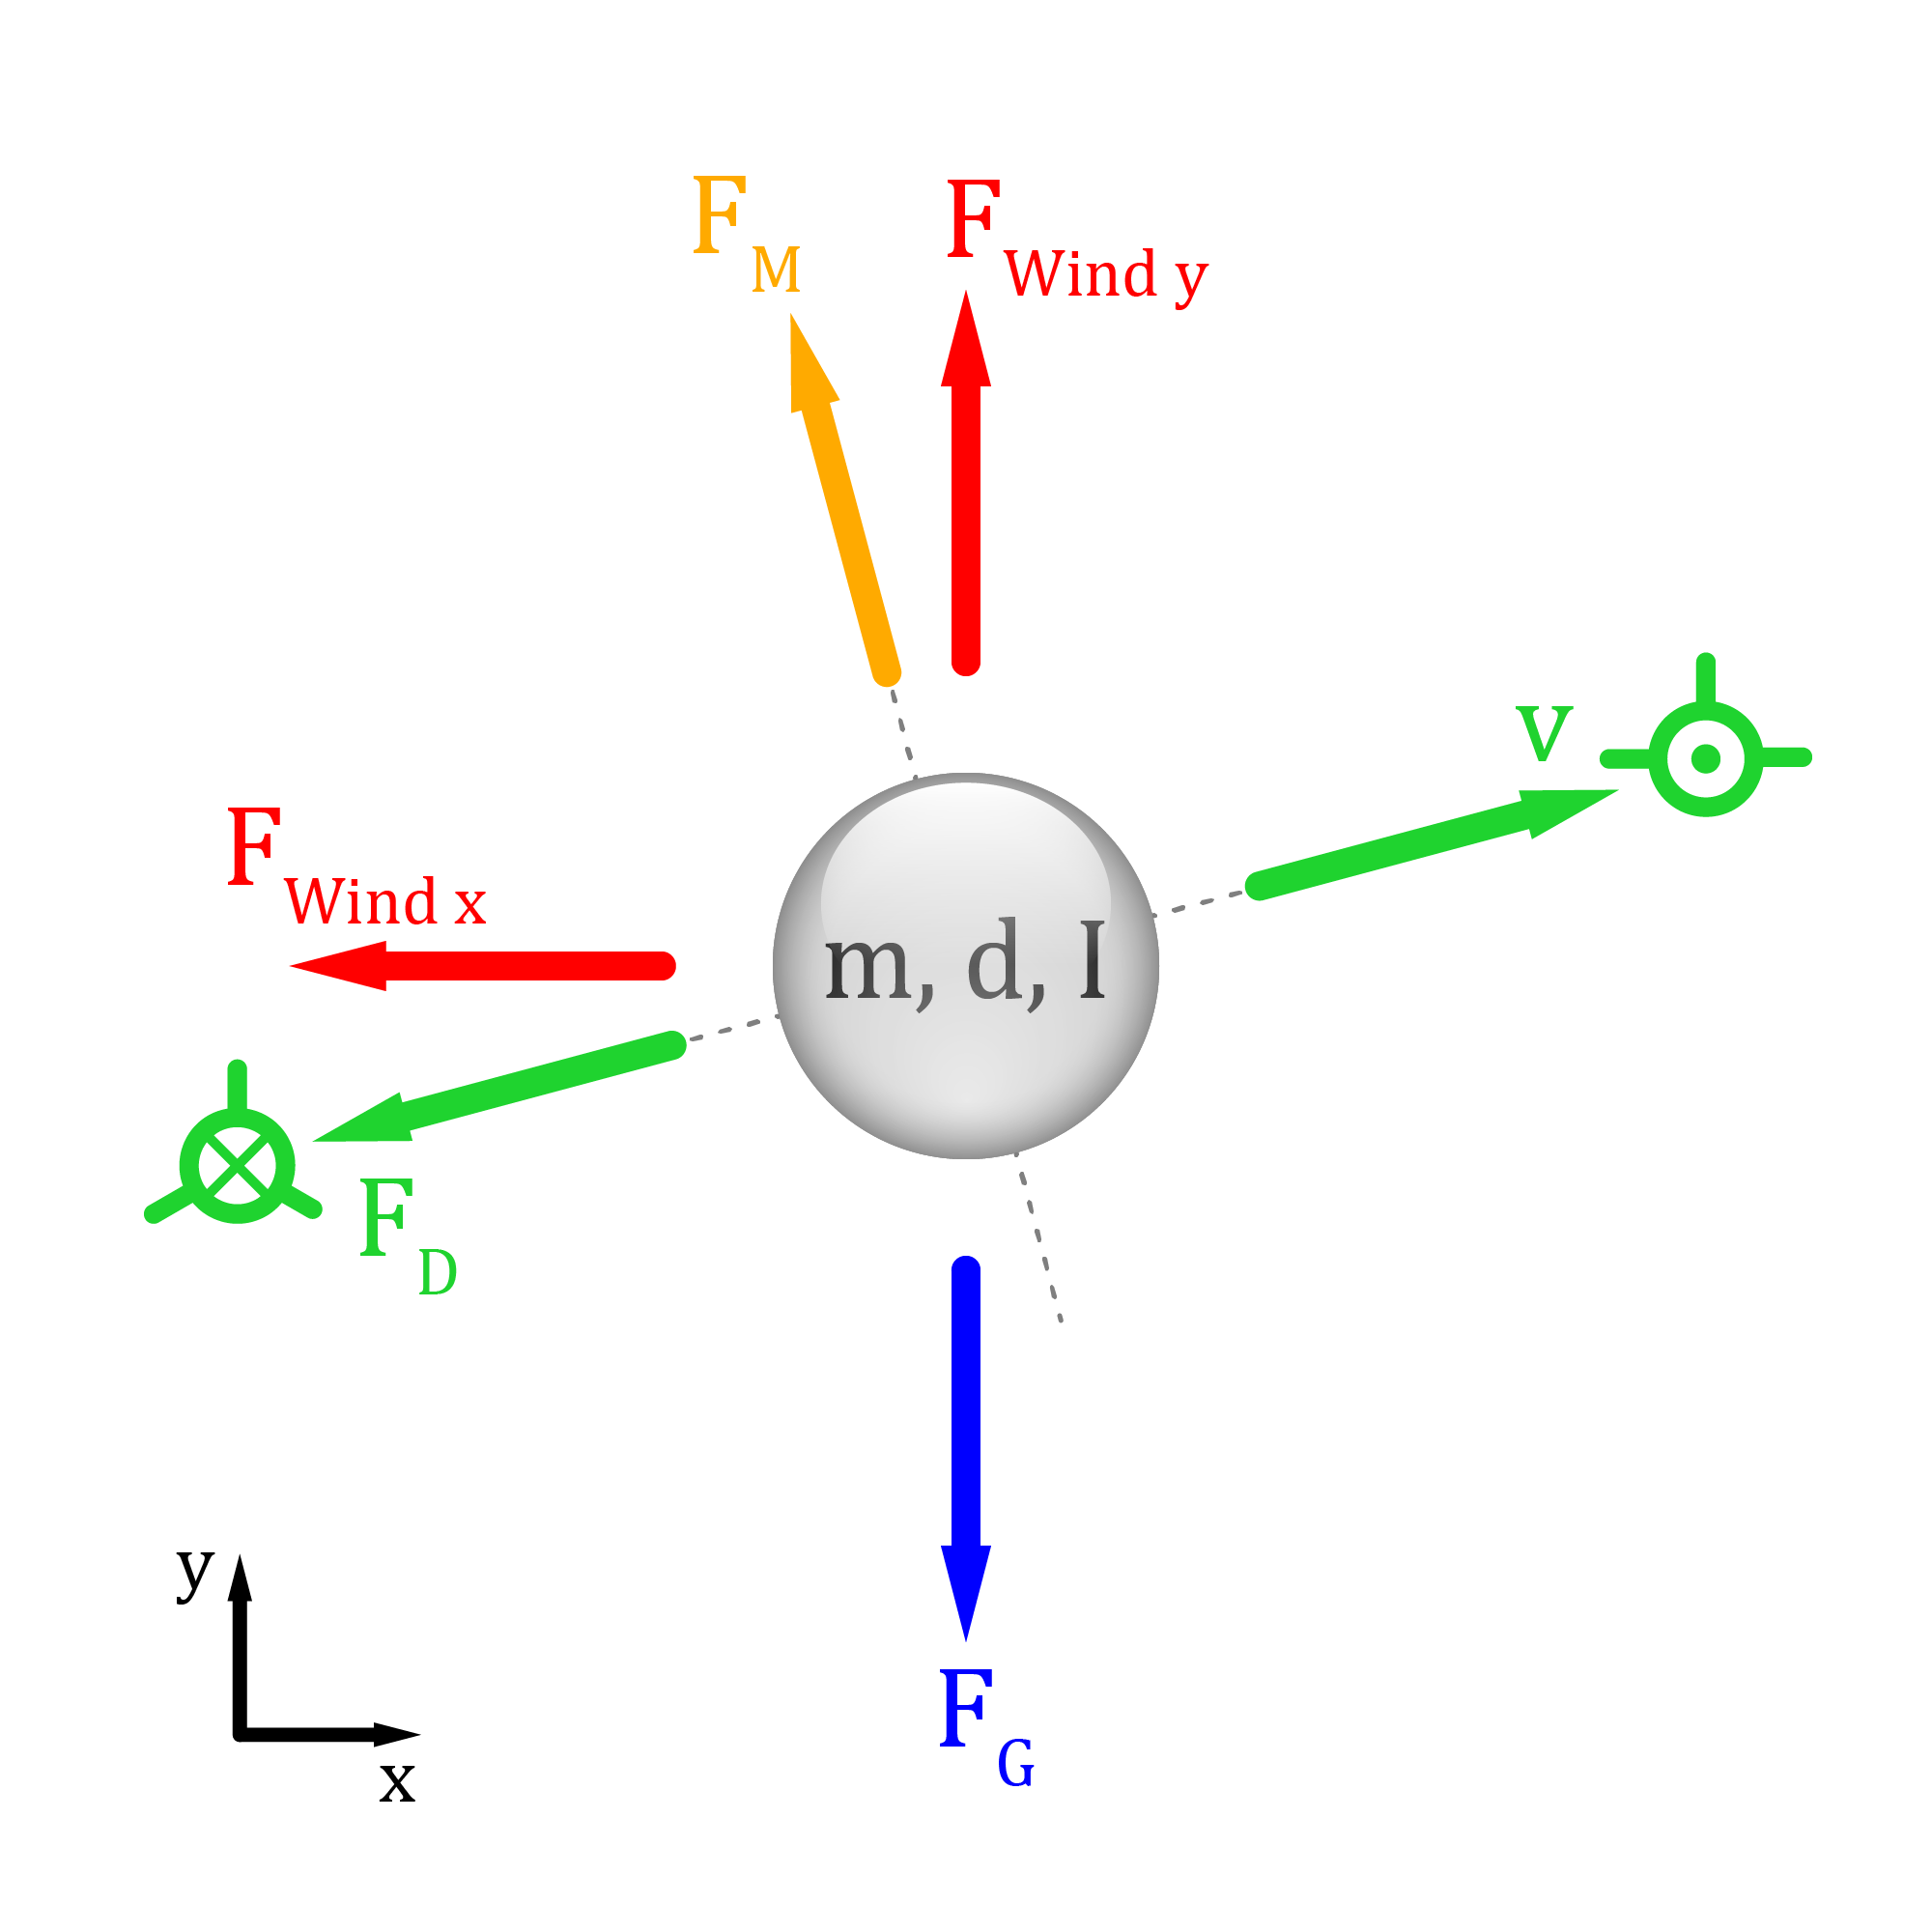
\includegraphics[width=0.4\textwidth]{airsoft_v3}\par
    \caption{Kräftediagramm} % Bildbeschreibung
\end{figure}

\subsubsection{Kräfte}

\subsection{Formeln zur Berechnung}

\begin{align}
    G&=2 \pi b V_{r}    \\
    V_{r}&=2 \pi b s \\
    L_{G}&= p(2 \pi r V_{r})*(2 \pi r \omega ) \\
    F_{Magnus}&= \lim \limits_{d \to 0} \sum\limits_{}^{r/d} F(d,r) \\
    F_{LR}&= \frac{1}{2} *A*c_{w}* \rho_{Luft}*v^2
\end{align}
(1) Wirbelstärke, (2) Rotationsgeschwindigkeit s = spin b = Radius des Zylinders\\
(3) Auftrieb durch Verdrängung von Luft, (4) Kraft des Magnuseffekts, (5) Luftwiderstand \\
Anmerkung: Die dargestellten Formeln repräsentieren den Teil des Simulationsumfangs der garantiert vorkommen wird. Im Laufe der Ausarbeitung können weitere Einflüsse berücksichtigt werden.

\subsection{Startparameter}

Die Startparameter sollen in der Simulation vom Endnutzer final in einer dafür passenden Bedienoberfläche eingegeben werden. 
Die Parameter beziehen sich auf das Gewicht der Kugel in Gramm, den Durchmesser der Kugel in Millimetern, die Abschussenergie in Joule, den Abschusswinkel in Grad, die Höhe, in der die Kugel abgeschossen wird in Metern, sowie die Einstellung der Rotationsgeschwindigkeit der Kugel.

\section{Softwareumfang der Ausarbeitung}

- Matlab App Designer für Benutzeroberfläche und Visualisierung\\
- Code und Berechnung über Matlab (eventuell werden noch andere Tools hinzugefügt)\\
- Overleaf für die Dokumentation

\centering

\end{document}
